\newpage
\chapter{TINJAUAN PUSTAKA} \label{Bab II}

\section{Tinjauan Pustaka} \label{II.Tinjauan}
Tinjauan pustaka ini memaparkan penelitian terdahulu yang memiliki relevansi topik dan menjadi landasan utama penyusunan tugas akhir. Adapun penelitian yang dijadikan acuan diuraikan sebagai berikut. \par

Zi dkk. pada tahun 2021 mempermasalahkan keterbatasan dataset \textit{deepfake} yang umumnya disusun dalam kondisi terkontrol, sehingga kurang merepresentasikan variasi konten dunia nyata yang beredar di internet \cite{Zi2024}. Untuk mengatasi hal tersebut, mereka memperkenalkan dataset WildDeepfake yang terdiri atas 7.314 \textit{face sequence} yang diekstraksi dari 707 video \textit{deepfake} yang dikumpulkan sepenuhnya dari internet \cite{Zi2024}. Kontribusi utama penelitian ini terletak pada penyediaan dataset \textit{in-the-wild} yang lebih menantang dibandingkan dataset terkontrol, serta evaluasi sejumlah detektor dasar yang menunjukkan penurunan performa yang cukup besar pada dataset tersebut \cite{Zi2024}. Bagi penelitian ini, paper tersebut menjadi landasan utama dalam pemilihan WildDeepfake sebagai sumber data, karena menunjukkan bahwa evaluasi model pada data terkontrol saja belum cukup untuk menggambarkan ketahanan model pada kondisi operasional yang sesungguhnya. \par

Khormali dan Yuan pada tahun 2022 mengangkat masalah bahwa sebagian besar metode deteksi \textit{deepfake} masih bergantung pada arsitektur CNN, yang dinilai kurang optimal dalam menangkap hubungan global antarbagi citra \cite{app12062953}. Mereka mengusulkan DFDT, yaitu kerangka \textit{end-to-end} berbasis Vision Transformer yang terdiri atas komponen \textit{patch extraction and embedding}, \textit{multi-stream transformer block}, \textit{attention-based patch selection}, dan \textit{multi-scale classifier} \cite{app12062953}. Hasil pengujian menunjukkan bahwa DFDT mencapai akurasi 99,41\% pada FaceForensics++, 99,31\% pada Celeb-DF (V2), dan 81,35\% pada WildDeepfake \cite{app12062953}. Penelitian ini relevan karena secara langsung mendukung penggunaan ViT pada pendekatan spasial untuk klasifikasi \textit{deepfake}. Selain itu, keberhasilan DFDT pada WildDeepfake menunjukkan bahwa Transformer berbasis citra tetap memiliki potensi yang baik pada data dunia nyata, sehingga layak dijadikan pembanding konseptual bagi pendekatan spasial yang digunakan dalam penelitian ini. \par

Zhuang dkk. pada tahun 2022 membahas permasalahan bahwa pembelajaran inkonsistensi pemalsuan wajah umumnya memerlukan anotasi lokasi manipulasi tingkat piksel, padahal anotasi semacam itu sulit diperoleh dan mahal dibuat \cite{zhuang2022uiavitunsupervisedinconsistencyawaremethod}. Untuk menjawab masalah tersebut, mereka mengusulkan UIA-ViT, yaitu metode berbasis ViT yang memanfaatkan \textit{self-attention} untuk mempelajari inkonsistensi intra-\textit{frame} hanya dengan label tingkat video, melalui dua komponen utama berupa \textit{Unsupervised Patch Consistency Learning} (UPCL) dan \textit{Progressive Consistency Weighted Assemble} (PCWA) \cite{zhuang2022uiavitunsupervisedinconsistencyawaremethod}. Kontribusi penelitian ini menunjukkan bahwa ViT tidak hanya efektif sebagai pengganti CNN, tetapi juga memiliki keunggulan metodologis dalam memodelkan relasi antarpetak citra yang relevan untuk mendeteksi inkonsistensi manipulasi \cite{zhuang2022uiavitunsupervisedinconsistencyawaremethod}. Bagi penelitian ini, UIA-ViT memperkuat justifikasi bahwa pendekatan spasial berbasis ViT masuk akal untuk diterapkan pada klasifikasi video \textit{deepfake}, karena informasi visual statis pada tingkat \textit{frame} masih dapat dieksploitasi secara efektif melalui mekanisme perhatian global. \par

Kingra dkk. tahun 2024 menyoroti bahwa banyak metode sebelumnya belum mampu memanfaatkan informasi spasial dan temporal secara terpadu dalam satu kerangka Transformer \textit{end-to-end} \cite{KINGRA2024301817}. Untuk itu, mereka mengusulkan SFormer yang menggunakan Swin Transformer untuk analisis spasial, diikuti \textit{transformer block} untuk analisis temporal, dan \textit{MLP block} untuk prediksi akhir \cite{KINGRA2024301817}. Hasil eksperimen menunjukkan bahwa SFormer memperoleh akurasi 100\% pada FF++, 97,81\% pada DFD, 99,1\% pada Celeb-DF, dan 93,67\% pada DFDC, serta menunjukkan kemampuan generalisasi yang baik pada eksperimen lintas-dataset \cite{KINGRA2024301817}. Penelitian ini relevan karena mendukung argumen bahwa pendekatan spasiotemporal berbasis Transformer merupakan arah yang kuat untuk deteksi \textit{deepfake} video. Dalam konteks penelitian ini, SFormer menjadi pembanding penting pada jalur spasiotemporal karena menunjukkan bahwa pemodelan hubungan antar-\textit{frame} dapat meningkatkan kemampuan model dalam menangkap jejak manipulasi yang tidak selalu tampak pada \textit{frame} tunggal. \par

Hu dkk. pada tahun 2024 membahas tantangan bahwa video \textit{deepfake} modern sering memiliki jejak manipulasi yang tersebar secara acak dan berubah antar-\textit{frame}, sehingga sulit dideteksi hanya dengan fitur lokal yang tetap \cite{hu2024delocatedetectionlocalizationdeepfake}. Mereka mengusulkan metode Delocate untuk deteksi dan lokalisasi \textit{deepfake}, serta melakukan studi \textit{ablation} yang secara langsung membandingkan MAE dan VideoMAE pada tugas deteksi \textit{deepfake} \cite{hu2024delocatedetectionlocalizationdeepfake}. Dalam \textit{ablation study} tersebut, baseline VideoMAE memperoleh skor AUC 77,4 pada CDF, 89,3 pada DFo, dan 71,8 pada DFDC, sementara Delocate menunjukkan peningkatan lebih lanjut setelah dilakukan modifikasi terhadap strategi pemodelan \cite{hu2024delocatedetectionlocalizationdeepfake}. Walaupun VideoMAE pada penelitian ini tidak digunakan sebagai metode utama oleh Hu dkk., keberadaan VideoMAE sebagai baseline yang dievaluasi secara langsung pada domain \textit{deepfake} tetap penting, karena menunjukkan bahwa representasi video berbasis Transformer sudah mulai digunakan dan relevan untuk tugas deteksi \textit{deepfake} video. Dengan demikian, paper ini dapat dijadikan justifikasi tambahan bagi pemilihan VideoMAE sebagai model pada pendekatan spasiotemporal dalam penelitian ini. \par

Berdasarkan lima penelitian tersebut, dapat disimpulkan bahwa terdapat tiga landasan utama yang mendukung penelitian ini. Pertama, WildDeepfake terbukti merupakan dataset yang lebih menantang dan lebih representatif untuk evaluasi pada kondisi dunia nyata \cite{Zi2024}. Kedua, pendekatan spasial berbasis ViT telah menunjukkan potensi yang baik dalam mendeteksi artefak visual statis pada \textit{deepfake} \cite{app12062953,zhuang2022uiavitunsupervisedinconsistencyawaremethod}. Ketiga, pendekatan spasiotemporal berbasis Transformer, termasuk model video seperti VideoMAE, menunjukkan potensi untuk menangkap bukti manipulasi yang tersebar pada dimensi spasial dan temporal \cite{KINGRA2024301817,hu2024delocatedetectionlocalizationdeepfake}. Meskipun demikian, masih terdapat celah penelitian berupa belum banyaknya studi yang secara langsung membandingkan pendekatan spasial berbasis ViT dan pendekatan spasiotemporal berbasis VideoMAE pada dataset WildDeepfake dalam satu rancangan eksperimen yang setara. Oleh karena itu, penelitian ini diarahkan untuk mengisi celah tersebut melalui analisis komparatif kedua pendekatan pada skenario \textit{deepfake in-the-wild}. \par

\begin{longtable}{|b{0.05\textwidth}|p{0.2\textwidth}|p{0.2\textwidth}|p{0.2\textwidth}|p{0.25\textwidth}|} % Longtable berguna agar tabel dapat terpotong di halaman baru
	\caption{Literasi Penelitian Terdahulu}
	\label{table:2.literasi}\\
	\hline
	\textbf{No.} & \textbf{Judul} & \textbf{Masalah} & \textbf{Metode} & \textbf{Hasil} \\
	\hline
	\endfirsthead % Header tabel untuk halaman pertama
	\hline
	\textbf{No.} & \textbf{Judul} & \textbf{Masalah} & \textbf{Metode} & \textbf{Hasil} \\
	\hline
	\endhead % Header tabel untuk halaman selanjutnya (repeat header row)
	1. & WildDeepfake: A Challenging Real-World Dataset for Deepfake Detection (Zi dkk., 2024) & Dataset \textit{deepfake} terkontrol kurang mewakili kondisi dunia nyata. & Memperkenalkan dataset WildDeepfake dan menguji beberapa baseline deteksi. & WildDeepfake lebih menantang daripada dataset terkontrol dan layak digunakan untuk evaluasi \textit{in-the-wild}.\\
	\hline
	2. & DFDT: An End-to-End DeepFake Detection Framework Using Vision Transformer (Khormali dkk., 2022) & CNN kurang optimal menangkap relasi global citra. & Mengusulkan deteksi \textit{deepfake} berbasis Vision Transformer. & Mencapai akurasi tinggi pada beberapa dataset, termasuk WildDeepfake, dan mendukung penggunaan ViT.\\
	\hline
	3. & UIA-ViT: Unsupervised Inconsistency-Aware Method based on Vision Transformer for Face Forgery Detection (Zhuang dkk., 2022) & Deteksi inkonsistensi manipulasi biasanya memerlukan anotasi piksel. & Menggunakan ViT untuk mempelajari inkonsistensi intra-\textit{frame} tanpa anotasi piksel. & Menunjukkan generalisasi yang baik dan memperkuat efektivitas ViT untuk deteksi manipulasi wajah.\\
	\hline
	4. & SFormer: An End-to-End Spatio-Temporal Transformer Architecture for Deepfake Detection (Kingra dkk., 2024) & Diperlukan model yang memanfaatkan informasi spasial dan temporal secara terpadu. & Menggunakan Swin Transformer dan \textit{transformer temporal} untuk deteksi video \textit{deepfake}. & Memberikan akurasi tinggi pada beberapa dataset dan mendukung pendekatan spasiotemporal berbasis Transformer.\\
	\hline
	5. & Delocate: Detection and Localization for Deepfake Videos with Randomly-Located Tampered Traces (Hu dkk., 2024) & Jejak manipulasi video \textit{deepfake} tersebar acak dan berubah antar-\textit{frame}. & Mengusulkan model deteksi-lokalisasi dan membandingkan baseline MAE dan VideoMAE. & Menunjukkan peningkatan deteksi lintas-domain dan mendukung relevansi VideoMAE pada deteksi \textit{deepfake} video.\\
	\hline
\end{longtable}

\section{Dasar Teori} \label{II.Teori}
\subsection{Deepfake dan Manipulasi Media Visual} \label{II.Teori1}
Perkembangan manipulasi media visual mengalami perubahan yang sangat signifikan seiring kemajuan \textit{deep learning}, khususnya pada model generatif yang mampu mensintesis wajah dan video dengan tingkat realisme yang tinggi. Dalam konteks ini, \textit{deepfake} dipahami sebagai salah satu bentuk media sintetis yang dihasilkan atau dimanipulasi menggunakan model berbasis jaringan saraf dalam, sehingga konten visual yang dihasilkan tampak autentik meskipun tidak sepenuhnya merepresentasikan kondisi yang sebenarnya \cite{Mirsky_2021}. Realisme \textit{deepfake} semakin meningkat setelah berkembangnya arsitektur generator modern yang mampu menghasilkan wajah sintetis beresolusi tinggi dengan detail tekstur, pencahayaan, dan struktur wajah yang semakin alami \cite{karras2019stylebasedgeneratorarchitecturegenerative}. Kondisi tersebut menyebabkan manipulasi media visual tidak lagi terbatas pada penyuntingan konvensional, tetapi telah berkembang menjadi rekayasa identitas, ekspresi, dan gerak wajah yang sulit dibedakan dari media asli \cite{Mirsky_2021,karras2019stylebasedgeneratorarchitecturegenerative}. \par

\subsubsection{Deepfake} \label{II.Teori1.1}
\textit{Deepfake} adalah media sintetis atau media yang dimanipulasi menggunakan teknik \textit{deep learning} untuk menghasilkan konten visual atau audiovisual yang menyerupai data asli secara sangat meyakinkan \cite{Mirsky_2021}. Dalam praktiknya, \textit{deepfake} tidak hanya mencakup pertukaran wajah (\textit{face swapping}), tetapi juga sintesis wajah penuh, manipulasi ekspresi wajah, rekayasa gerak bibir, dan perubahan identitas visual pada video \cite{Mirsky_2021}. Karakteristik utama \textit{deepfake} terletak pada kemampuannya mempertahankan kesan visual yang realistis bagi pengamat manusia, sehingga media hasil manipulasi tampak sah secara visual walaupun tidak autentik secara semantik \cite{Mirsky_2021}. Oleh karena itu, \textit{deepfake} menjadi salah satu bentuk manipulasi media visual yang paling menantang dalam bidang forensik digital, karena kualitas hasil generasinya terus meningkat seiring perkembangan model generatif modern \cite{Mirsky_2021,karras2019stylebasedgeneratorarchitecturegenerative}. \par

\subsubsection{Konsep dan Generasi Deepfake} \label{II.Teori1.2}
Konsep generasi \textit{deepfake} sangat erat kaitannya dengan perkembangan model generatif, terutama \textit{Generative Adversarial Networks} (GAN). GAN merupakan kerangka pembelajaran generatif yang melibatkan dua jaringan, yaitu \textit{generator} yang bertugas menghasilkan sampel sintetis dan \textit{discriminator} yang bertugas membedakan sampel sintetis dari data asli \cite{NIPS2014_f033ed80}. Melalui proses pelatihan yang bersifat \textit{adversarial}, \textit{generator} secara bertahap belajar menghasilkan data yang semakin menyerupai distribusi data nyata \cite{NIPS2014_f033ed80}. Kerangka ini menjadi fondasi penting bagi generasi awal \textit{deepfake} karena memungkinkan pembentukan wajah sintetis dan manipulasi visual berbasis data dengan kualitas yang terus meningkat. Perkembangan berikutnya menghasilkan arsitektur yang lebih kuat, salah satunya \textit{style-based generator architecture} pada StyleGAN, yang memungkinkan kontrol yang lebih baik terhadap atribut visual tingkat tinggi seperti identitas, pose, dan struktur wajah, sekaligus mempertahankan detail lokal yang halus \cite{karras2019stylebasedgeneratorarchitecturegenerative}. Dengan demikian, realisme \textit{deepfake} modern tidak hanya ditentukan oleh kemampuan menghasilkan wajah yang tampak alami, tetapi juga oleh kemampuan model dalam menjaga konsistensi detail visual sehingga artefak manipulasi menjadi semakin sulit dikenali \cite{NIPS2014_f033ed80,karras2019stylebasedgeneratorarchitecturegenerative}. \par

\subsubsection{Karakteristik Dataset In-the-Wild} \label{II.Teori1.3}
Karakteristik dataset \textit{in-the-wild} berbeda secara mendasar dari dataset yang dibangun dalam kondisi terkontrol. Pada data terkontrol, video umumnya memiliki kualitas yang lebih seragam, resolusi yang relatif stabil, pencahayaan yang lebih terkendali, dan tingkat kompresi yang tidak terlalu beragam. Sebaliknya, dataset \textit{in-the-wild} merepresentasikan kondisi distribusi dunia nyata yang jauh lebih kompleks, karena memuat variasi kompresi, resolusi, pencahayaan, pose, ekspresi, latar belakang, sudut pengambilan gambar, serta kualitas video yang tidak seragam \cite{Zi2024,li2020celebdflargescalechallengingdataset}. Perbedaan tersebut menyebabkan jejak manipulasi pada video \textit{deepfake} menjadi lebih sulit dikenali dibandingkan pada dataset terkontrol. Pergeseran menuju dataset yang lebih realistis juga terlihat pada Celeb-DF, yang dirancang sebagai dataset \textit{DeepFake} yang lebih menantang dengan kualitas visual yang lebih tinggi daripada dataset generasi awal \cite{li2020celebdflargescalechallengingdataset}. Pada konteks yang lebih luas, WildDeepfake merepresentasikan karakteristik \textit{in-the-wild} secara lebih kuat karena disusun dari video yang benar-benar dikumpulkan dari internet dan menunjukkan bahwa performa detektor dasar dapat menurun cukup drastis ketika diuji pada kondisi dunia nyata \cite{Zi2024}. Oleh karena itu, karakteristik utama dataset \textit{in-the-wild} dalam penelitian ini dipahami sebagai keberagaman kondisi visual dan degradasi nyata yang membuat proses klasifikasi \textit{deepfake} menjadi lebih menantang daripada pada data yang dibangun dalam lingkungan terkontrol \cite{Zi2024,li2020celebdflargescalechallengingdataset}. \par

\subsection{Deep Learning} \label{II.Teori2}
\textit{Deep learning} adalah cabang dari \textit{machine learning} yang menggunakan jaringan saraf tiruan berlapis banyak untuk mempelajari representasi data secara bertingkat, mulai dari pola berlevel rendah hingga representasi berlevel tinggi yang lebih abstrak \cite{LeCun2015}. Pendekatan ini memungkinkan proses ekstraksi fitur dilakukan secara otomatis dari data, sehingga mengurangi ketergantungan pada perancangan fitur manual yang umum digunakan pada metode pembelajaran tradisional \cite{LeCun2015}. Dalam perkembangannya, \textit{deep learning} telah menunjukkan peningkatan kinerja yang signifikan pada berbagai tugas, seperti pengenalan ucapan, pengenalan objek visual, deteksi objek, dan analisis data berskala besar \cite{LeCun2015}. Pada konteks penelitian ini, \textit{deep learning} menjadi landasan utama dalam pembangunan model klasifikasi video \textit{deepfake}, karena pendekatan ini memungkinkan model mempelajari pola visual yang kompleks dari citra wajah dan klip video secara langsung dari data \cite{LeCun2015,Voulodimos2018}. \par

\subsection{Computer Vision} \label{II.Teori3}
\textit{Computer vision} adalah bidang dalam kecerdasan buatan yang berfokus pada bagaimana sistem komputer memperoleh, merepresentasikan, dan memahami informasi dari citra maupun video \cite{Voulodimos2018}. Perkembangan \textit{deep learning} telah mendorong kemajuan pesat pada bidang ini, terutama pada tugas klasifikasi citra, deteksi objek, segmentasi, dan analisis visual lainnya, karena model dapat mempelajari fitur visual secara lebih efektif dibandingkan pendekatan konvensional \cite{Voulodimos2018}. Dalam penelitian ini, \textit{computer vision} menjadi kerangka aplikasi yang mendasari proses analisis \textit{face sequence} dan klip video untuk membedakan konten \textit{real} dan \textit{fake} berdasarkan karakteristik visual yang dipelajari model \cite{Voulodimos2018}. Dengan demikian, \textit{computer vision} tidak hanya berperan sebagai domain penerapan, tetapi juga sebagai dasar konseptual dalam memahami bagaimana informasi visual pada video \textit{deepfake} dapat diolah menjadi keputusan klasifikasi \cite{Voulodimos2018}. \par

\subsection{Transformer} \label{II.Teori4}
Transformer merupakan arsitektur jaringan saraf yang diperkenalkan untuk memodelkan hubungan antar elemen masukan melalui mekanisme \textit{attention} tanpa bergantung pada proses rekuren maupun konvolusi \cite{vaswani2023attentionneed}. Berbeda dengan \textit{Recurrent Neural Network} (RNN) dan \textit{Long Short-Term Memory} (LSTM) yang memproses data secara berurutan, Transformer memungkinkan setiap elemen masukan berinteraksi secara langsung dengan elemen lainnya dalam satu urutan, sehingga konteks global dapat dipelajari secara lebih efektif \cite{vaswani2023attentionneed}. Karakteristik ini membuat Transformer menjadi salah satu fondasi utama dalam perkembangan \textit{deep learning} modern dan kemudian diadaptasi ke berbagai domain, tidak hanya pada \textit{Natural Language Processing} (NLP), tetapi juga pada \textit{computer vision} \cite{vaswani2023attentionneed}. \par

Secara umum, arsitektur Transformer terdiri atas blok \textit{encoder} dan \textit{decoder} yang dibangun dari komponen utama berupa \textit{multi-head attention}, \textit{feed-forward network}, \textit{residual connection}, dan \textit{layer normalization} \cite{vaswani2023attentionneed}. Pada penelitian ini, konsep Transformer menjadi dasar penting karena baik \textit{Vision Transformer} (ViT) maupun VideoMAE sama-sama memanfaatkan mekanisme perhatian untuk membangun representasi visual dari citra dan video \cite{dosovitskiy2021imageworth16x16words,tong2022videomaemaskedautoencodersdataefficient,vaswani2023attentionneed}. Dengan demikian, pemahaman terhadap Transformer diperlukan untuk menjelaskan bagaimana hubungan global antarbagian masukan visual dapat dipelajari secara langsung tanpa ketergantungan pada struktur rekuren maupun operasi konvolusi tradisional. \par

Mekanisme inti pada Transformer adalah \textit{self-attention}, yaitu proses yang memungkinkan setiap elemen masukan memberikan perhatian terhadap elemen lainnya dalam urutan yang sama \cite{vaswani2023attentionneed}. Pada mekanisme ini, setiap elemen masukan diproyeksikan ke dalam tiga representasi, yaitu \textit{Query} (Q), \textit{Key} (K), dan \textit{Value} (V). Hubungan antar elemen dihitung melalui perkalian antara Q dan K untuk memperoleh skor kesamaan, kemudian dinormalisasi dengan fungsi \textit{softmax} agar diperoleh bobot perhatian yang proporsional \cite{vaswani2023attentionneed}. Bobot tersebut selanjutnya digunakan untuk menggabungkan V dan menghasilkan representasi baru yang telah memuat informasi konteks secara menyeluruh. Secara matematis, mekanisme ini dinyatakan sebagai berikut \cite{vaswani2023attentionneed}.

\vspace{0.6\baselineskip}
\begingroup
\begin{equation}
\mathrm{Attention}(Q, K, V) = \mathrm{softmax}\left(\frac{QK^{T}}{\sqrt{d_k}}\right)V
\label{eq:self-attention}
\end{equation}
\endgroup
\vspace{0.6\baselineskip}

Pada persamaan tersebut, Q, K, dan V merupakan matriks hasil transformasi linier dari masukan, sedangkan $d_k$ menyatakan dimensi vektor \textit{key} \cite{vaswani2023attentionneed}. Pembagian dengan $\sqrt{d_k}$ dilakukan untuk menstabilkan hasil perkalian \textit{dot product} agar nilainya tidak terlalu besar sebelum dinormalisasi oleh \textit{softmax} \cite{vaswani2023attentionneed}. Dengan mekanisme tersebut, Transformer mampu mempelajari hubungan kontekstual antar seluruh elemen masukan, bukan hanya elemen yang berdekatan. Arsitektur umum Transformer ditunjukkan pada Gambar \ref{fig:arsitektur-transformer}. \par

\begin{figure}[htbp]
	\centering
	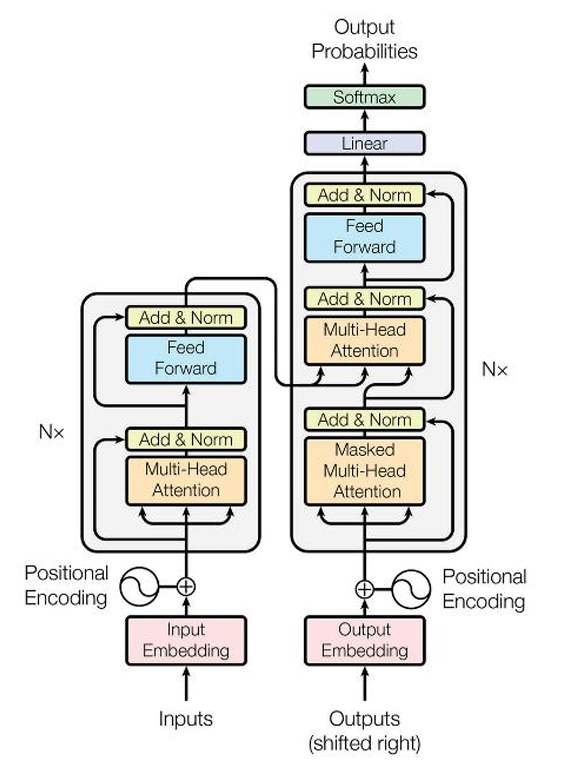
\includegraphics[width=0.5\textwidth]{figure/arsitektur-transformer.png}
	\caption{Arsitektur Transformer}
	\label{fig:arsitektur-transformer}
\end{figure}

\subsection{Vision Transformer (ViT)} \label{II.Teori5}
\textit{Vision Transformer} (ViT) merupakan adaptasi arsitektur Transformer untuk tugas klasifikasi citra dengan memproses citra sebagai urutan \textit{image patch} \cite{dosovitskiy2021imageworth16x16words}. Berbeda dengan \textit{Convolutional Neural Network} (CNN) yang menekankan ekstraksi fitur lokal melalui operasi konvolusi, ViT membagi citra menjadi sejumlah \textit{patch} dua dimensi, kemudian memperlakukan setiap \textit{patch} sebagai token masukan yang serupa dengan token pada pemrosesan bahasa alami \cite{dosovitskiy2021imageworth16x16words}. Pendekatan ini memungkinkan model memanfaatkan \textit{self-attention} untuk mempelajari hubungan global antarbagian citra secara langsung \cite{dosovitskiy2021imageworth16x16words}. Dalam konteks penelitian ini, ViT menjadi dasar pada pendekatan spasial karena setiap \textit{frame} video \textit{deepfake} diproses sebagai citra tunggal untuk mengekstraksi artefak visual statis. \par

Pada tahap awal pemrosesan, citra masukan berukuran $H \times W \times C$ dibagi menjadi sejumlah \textit{patch} berukuran $P \times P$ \cite{dosovitskiy2021imageworth16x16words}. Banyaknya \textit{patch} yang dihasilkan dinyatakan sebagai $N = \frac{HW}{P^2}$, sehingga citra tidak lagi diproses sebagai matriks piksel utuh, melainkan sebagai urutan token visual \cite{dosovitskiy2021imageworth16x16words}. Setiap \textit{patch} kemudian diratakan menjadi vektor satu dimensi dan diproyeksikan secara linier ke dalam ruang \textit{embedding} untuk membentuk \textit{patch embedding} \cite{dosovitskiy2021imageworth16x16words}. Setelah itu, sebuah \textit{class token} ditambahkan pada awal urutan token sebagai representasi global untuk keperluan klasifikasi, sedangkan \textit{positional embedding} ditambahkan untuk mempertahankan informasi posisi spasial tiap \textit{patch} \cite{dosovitskiy2021imageworth16x16words}. Dengan rancangan tersebut, citra dapat diproses oleh rangkaian Transformer \textit{encoder} dengan prinsip yang serupa dengan pengolahan token pada NLP. \par

Urutan token hasil \textit{embedding} selanjutnya diproses oleh Transformer \textit{encoder} yang tersusun atas blok \textit{multi-head self-attention} dan \textit{multi-layer perceptron} (MLP), disertai \textit{layer normalization} dan \textit{residual connection} \cite{dosovitskiy2021imageworth16x16words}. Melalui mekanisme ini, ViT mampu membangun representasi visual yang tidak hanya menangkap detail lokal, tetapi juga keterkaitan global antararea citra \cite{dosovitskiy2021imageworth16x16words}. Karakteristik tersebut menjadikan ViT relevan untuk klasifikasi \textit{deepfake}, karena manipulasi wajah pada \textit{deepfake} sering menghasilkan artefak visual yang tersebar pada berbagai bagian wajah dan tidak selalu terbatas pada pola lokal tertentu. Oleh karena itu, ViT memiliki dasar teoritis yang kuat untuk digunakan sebagai model pada pendekatan spasial dalam penelitian ini. Arsitektur \textit{Vision Transformer} ditunjukkan pada Gambar \ref{fig:arsitektur-vit}. \par

\begin{figure}[htbp]
	\centering
	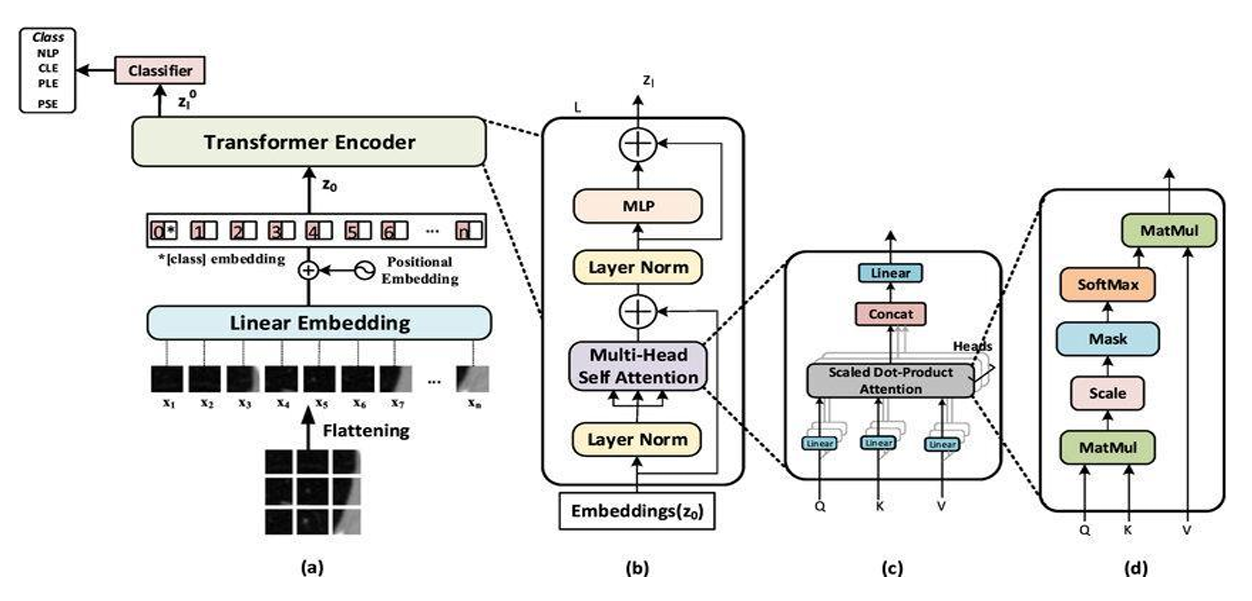
\includegraphics[width=0.9\textwidth]{figure/arsitektur-vision-transformer.png}
	\caption{Arsitektur Vision Transformer (ViT)}
	\label{fig:arsitektur-vit}
\end{figure}